\cotefile{156-7}
\scanpage{2}
\mspage{1}
\margin{\tikz[baseline=(h.base)]{\node[inner sep=2pt] (h) {\unsure{GF|CF} VII}; \draw (h.north west)--(h.south west)--(h.south east);}}
\begin{center}Analysis Situs (third version)\end{center}
% slanted
\margin{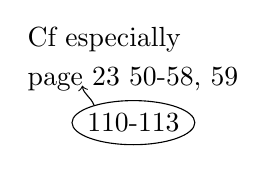
\begin{tikzpicture}[baseline=(n.base),x=1cm,y=1cm]
\node[anchor=west,inner sep=0pt] (n) at (0,0) {Cf especially};
\node[anchor=west,inner sep=0pt] at (0,-0.5) {page 23 \unsure{50}-\unsure{58}, 59};
\node[inner sep=1pt] (r) at (1.35,-1.05) {110-113};
\draw (1.35,-1.05) ellipse (0.78 and 0.28);
\draw[->] (0.85,-0.83) to[out=110,in=-80] (0.70,-0.58);
\end{tikzpicture}}

\uline{23 June}

I recapitulate the data and axioms of an ``algebra of figures'', or ``\uline{workshop}''. For the moment it is a matter of purely ``algebraic'' axioms governing the algebraic formalism of figures, to the exclusion for the moment of topological properties (density, connectedness, acyclicity) or \inserted{properly} geometric ones (topological regularity, topological balls and spheres of an algebra of figures), or even the ``fine combinatorial properties'', around the notion of \unsure{simplex|simplices|simplex}.

Among the axioms, I distinguish the ``sine qua non'' axioms At~1 to At~7, which seem to me the most essential for grounding the geometrico-topological meaning of the formalism envisaged. The other axioms will be considered as more or less ``optional'' at the level of the algebraic formalism. They \unsure{will be able to|could|could} \unsure{without|therefore}, \unsure{doubt|therefore|in} a crucial role, as soon as it is a matter of work on actual cases in the
